\documentclass[UTF8]{ctexart}

\usepackage[utf8]{inputenc}
\usepackage{lmodern}
\usepackage{amsmath}
\usepackage{amsfonts}
\usepackage{cite}
\usepackage{xcolor}
\usepackage{listings}
\usepackage{graphicx}
\usepackage{float}
\usepackage{multirow}
\usepackage{booktabs}
\usepackage{natbib}

% 定义颜色
\definecolor{codegreen}{rgb}{0,0.6,0}
\definecolor{codegray}{rgb}{0.5,0.5,0.5}
\definecolor{codeorange}{rgb}{1,0.49,0}
\definecolor{backcolour}{rgb}{0.95,0.95,0.96}

\renewcommand\lstlistingname{源代码}
\renewcommand\lstlistlistingname{源代码}

\lstdefinestyle{mystyle}{
backgroundcolor=\color{backcolour},   % Background color
commentstyle=\color{codegray},        % Comment color
keywordstyle=\color{codeorange},      % Keyword color
numberstyle=\tiny\color{codegray},    % Line number style
stringstyle=\color{codegreen},        % String style
basicstyle=\ttfamily\footnotesize,    % Basic font style and size
breakatwhitespace=false,              % Prevent line breaks at whitespace
breaklines=true,                      % Enable automatic line breaking
captionpos=b,                         % Caption position (bottom)
keepspaces=true,                      % Preserve spaces
numbers=left,                         % Line numbers on the left
numbersep=5pt,                        % Spacing between numbers and code
showspaces=false,                     % Do not show spaces as special characters
showstringspaces=false,               % Do not show spaces in strings as special characters
showtabs=false,                       % Do not show tabs as special characters
tabsize=2,                            % Tab size (spaces per tab)
xleftmargin=10pt                      % Left margin for the code block
}

\lstset{style=mystyle} % Apply the custom style

% 补充定义关键词函数
\providecommand{\keywords}[1]{
\small
\textbf{关键词:} #1
}

\title{一种基于的GAN的人脸图像生成技术探索}
\author{大数据2201 万方}
\date{\today}

\begin{document}

\maketitle
lll
\begin{abstract}
在人工智能技术蓬勃发展的今天,图像处理与分析已经成为学术界的热门研究领域。随着Stable Diffusion、Sora等生成式模型的火爆,图像生成的算法框架创新成为焦点问题。本文主要通过复现生成式对抗网络\\(GAN),探讨其原理和设计思想。作为创新贡献,本研究对GAN进行了优化,提出了改进的损失函数设计,调整了激活函数,并引入了卷积层来提升模型的生成效果。通过这些调整,本文期望能够在保持生成质量的基础上,进一步提升图像生成的稳定性和多样性,为图像生成技术的发展提供新的思路和参考。
\end{abstract}
\keywords{卷积神经网络(CNN),生成式对抗网络(GAN),图像生成,深度学习(DL)}
\section{引言}
图像生成技术在社会中的需求日益增加,尤其在创意产业、医疗、教育和娱乐等领域。静态图像生成技术最初通过生成对抗网络(GANs)和变分自编码器(VAEs)应用于艺术创作和广告设计,随着技术发展,从RNN到RNN+CNN,再到纯Diffusion模型,生成的图像质量和多样性不断提高。DiT(扩散型Transformer)等新兴模型则进一步优化了生成效果。视频生成领域中,VAR(视觉自回归模型)推动了视频内容的自动生成和编辑,应用于影视制作和虚拟现实等场景。此外,在医学领域,图像生成技术为医学影像的教学和科普提供了强有力的支持,降低了实际操作的风险。整体来看,图像生成技术正在促进各行各业的数字化转型,推动教育、创作和信息传播等多个领域的发展。
\subsection{图像生成领域的最新进展}
静态图像生成技术的发展历程可以追溯到深度学习方法的逐步演变,从卷积神经网络(CNN)到生成对抗网络(GAN),再到扩散模型(Diffusion)以及最新的结合了视觉自回归和Transformer结构的模型。\par
早期的静态图像生成主要依赖于CNN,通过自动编码器等方法进行图像重建和生成。CNN在图像处理中的成功为图像生成技术奠定了基础,它能够有效提取图像的空间特征,并生成具有较好视觉效果的图像。\par
接着,生成对抗网络(GAN)在2014年由Ian Goodfellow等提出,迅速成为图像生成领域的核心技术。GAN通过生成器与判别器的对抗训练,使得生成模型能够生成更加真实且细腻的图像。与传统的图像生成方法相比,GAN在生成效果和创新性上取得了显著突破,成为图像生成领域的重要里程碑。\par
随着研究的深入,Diffusion模型作为一种新兴的图像生成方法得到了广泛关注。\\Diffusion模型的核心思想是通过模拟噪声的逐步去除过程,从随机噪声中恢复出真实图像,能随着研究的深入,Diffusion模型作为一种新兴的图像生成方法逐渐引起了广泛关注。Diffusion模型的核心思想源于物理中的扩散过程,即通过逐步加入噪声,使图像变得模糊,然后再通过反向过程去噪声,逐渐恢复出原始图像。这种逐步去噪的过程在生成高质量图像方面表现出了强大的优势,相比于传统的生成对抗网络(GAN),Diffu-\\sion模型能够在生成细节和图像的真实性方面取得更好的效果。具体而言,Diffusion模型采用的是逐步迭代的方式进行图像恢复,这使得它在细节处理、纹理生成以及复杂图像的捕捉上具备了独特优势。通过大规模的训练数据集,Diffusion模型能够捕捉到图像中的微小细节,从而生成具有高度真实感的图像。\par
Diffusion模型和VAE(变分自编码器)的结合进一步推动了图像生成技术的进步。VAE作为一种生成模型,通过最大化变分下界来学习潜在变量的分布,从而在生成新样本时具备一定的潜力和泛化能力。VAE模型在生成过程中通过引入潜在空间的结构,使得生成的样本可以从潜在空间中进行平滑采样。然而,VAE的生成效果在精细度和图像细节上相对较弱,这限制了其在高质量图像生成中的应用。够生成高质量的图像,并且在处理细节方面优于传统GAN。随着VAE和Diffusion\\模型的结合,新的生成模型在生成质量和多样性方面进一步提高,具备了更强的泛化能力和更加精细的控制能力,使得生成的图像不仅更加多样化,同时也能在更广泛的潜在空间中进行高效的探索。而Diffusion模型的逐步去噪过程则增强了生成的图像质量,使得最终的输出更加精细且真实。通过这种结合,新的生成模型在生成质量、细节处理、潜在空间的控制能力及泛化能力方面得到了显著提升,能够生成更加符合语义要求且具备高保真度的图像。\par
最新的研究引入了Diffusion Transformer模型,它结合了Transformer结构的优势,引入了全流程语义引导,使得生成的图像更加符合语义表达并具备更好的上下文理解能力。这一进展使得图像生成不再局限于单纯的像素级优化,能够在更高层次上进行语义级的控制与生成,推动了图像生成技术向更加智能化、个性化的方向发展。\par
尽管Diffusion模型和Transformer结构近年来取得了显著进展,研究GAN依然具有重要价值。首先,GAN在生成速度、样本效率以及潜在空间的控制方面仍然具备一定的优势。此外,GAN的生成机制与传统的生成模型有着本质不同的对抗训练方式,这为研究生成模型的理论框架提供了丰富的灵感。通过进一步改进GAN的稳定性、训练技巧以及结合其他模型的优势,GAN依然是图像生成领域中一个重要的研究方向,尤其在生成速度和创意性方面,仍然是不可忽视的存在。
\subsection{图像工程手段在优化图像生成中的意义}

图像生成领域的优化不仅仅依赖于模型结构的创新,图像工程手段的引入也发挥着至关重要的作用。通过对图像数据进行适当的处理和优化,可以显著提高生成模型的效果和稳定性,促进更高质量图像的生成。以下是几种常见的图像工程手段及其对图像生成领域的优化意义。
\subsubsection{图像浮点化}
图像浮点化是将图像的像素值从整数转换为浮动的浮点数值,通常范围在[0, 1]之间。这一过程有助于提升生成模型对细节的捕捉能力,尤其是在训练过程中,浮点数能够提供更高的数值精度,使得模型能够更好地处理图像中的细微差别。浮点化的图像数据在训练过程中能够减少数值溢出问题,提高模型的收敛性和稳定性,尤其对于深度神经网络而言,精确的数值操作是确保高质量生成的基础。
\subsubsection{图像归一化}
图像归一化通常指将图像的像素值按某种方式进行缩放,使其分布符合一定的标准,比如将像素值规范化到0到1之间,或对每个通道进行零均值和单位方差的归一化。归一化的作用是加速模型的训练过程,使得梯度更新更加稳定,避免了过大的或过小的数值导致的梯度消失或梯度爆炸问题。此外,归一化还能够帮助神经网络更好地学习图像的全局特征,尤其是对于复杂图像的生成任务,归一化提供了数据预处理的标准化,从而提高了图像生成的质量和训练效率。
\subsubsection{引入卷积方法}
卷积神经网络(CNN)是图像生成中不可或缺的组件。CNN通过卷积操作能够有效地捕捉图像的局部特征,并提取出从低级到高级的层次特征。在图像生成过程中,引入卷积方法使得生成网络能够从原始图像中自动学习到有效的特征,不需要手动设计特征提取器。卷积方法不仅能够提升图像生成的效率,还能增强模型对于图像局部细节的处理能力,从而生成更加细腻、真实的图像。
\subsubsection{激活函数调优}
激活函数在神经网络中的作用是引入非线性,使得网络能够学习到更复杂的映射关系。常见的激活函数如ReLU、Leaky ReLU、Sigmoid、$tanh$等,各自具有不同的特性。通过对激活函数的选择和调优,能够显著影响生成模型的表现。
例如,ReLU(Rectified Linear Unit)及其变种Leaky ReLU在图像生成中得到了广泛应用,因为它们能够有效避免梯度消失问题,并在深层网络中保证更快的训练速度。然而,ReLU在负值输入时会“死亡”(即输出为零),因此在某些任务中,调优激活函数的选择能有效解决这一问题,从而提高模型的生成能力。

\subsubsection{综合影响}
这些图像工程手段的优化有助于提升图像生成任务中的多个维度,首先是提升生成图像的质量,使得模型能够更加精细地还原原图像的细节;其次,优化数据处理方式能够加速训练过程,减少训练时可能出现的数值问题;最后,通过结合适当的卷积操作和激活函数,能够增强模型的表达能力,使其能够生成更多样化和更具创意的图像。整体而言,图像工程手段的优化为图像生成领域提供了更加稳定和高效的训练框架,也为高质量图像生成提供了必要的支持。这些技术的结合,不仅提升了生成模型的性能,也为更复杂、更具有挑战性的生成任务(如高分辨率图像生成、特定样式图像生成等)奠定了坚实的基础。而本研究也将从向


\subsection{本研究的价值}

研究在图像生成领域具有一定的创新价值。通过复现生成对抗网络(GAN),我深入探讨了其原理和设计思想,并基于此进行了优化。具体来说,我提出了改进的损失函数设计,调整了激活函数,并引入了卷积层,以提升模型的生成效果。这些优化有助于解决传统GAN在训练过程中常遇到的稳定性问题,并有效避免了模式崩溃现象。通过这些调整,模型能够在保持高质量生成图像的基础上,显著提高生成的稳定性和多样性。

此外,卷积层的引入使得模型在处理图像的局部特征时更加高效,能够生成更加细腻、真实的图像。这不仅增强了图像的细节表现,也提升了整体生成质量。在保证图像质量的同时,我还进一步增强了生成图像的多样性,有效避免了生成结果的单一性。这些改进为图像生成技术提供了新的思路,并推动了其在实际应用中的发展,特别是在需要生成高质量、多样化图像的场景中。
综上所述,本研究通过对GAN模型的优化,为图像生成技术的稳定性和多样性提供了有效的提升方案,为相关领域的学术研究和实际应用提供了新的参考和思路。
\subsection{使用的数据集}
LFW(Labeled Faces in the Wild)数据集是一个广泛使用的人脸识别数据集,包含了13233张来自5000多个不同人的人脸图像。每张图像的大小为250x250像素(在本文中使用OpenCV模块放缩至125x125以降低运算量),并且具有多样的姿势、表情和背景。通过利用GAN训练一个生成器,能够自动生成出与 LFW 数据集中的真实人脸相似的假人脸图像。由于 DCGAN 在图像生成任务中的优异表现,它被选为本次实验的基础架构。
\section{方法}
\subsection{GAN的结构与设计}
生成对抗网络(GAN)是由Ian Goodfellow及其团队于2014年提出的一种生成模型,其设计思想源于博弈论的“零和博弈”(Zero-Sum Game)。在GAN中,生成器(Generator)和判别器(Discriminator)构成了一个对抗的博弈系统,通过两者相互博弈来不断优化生成图像的质量。GAN的核心思想是利用生成器和判别器之间的对抗训练,推动生成器生成越来越真实的数据,最终使生成器生成的数据与真实数据无法区分。
GAN模型的核心设计思想是将生成器和判别器看作对立的两方,它们通过博弈的方式共同训练。生成器的目标是生成逼真的数据,以便能骗过判别器,而判别器的目标是能够区分出真实数据和生成数据。二者的训练过程是交替进行的,生成器通过不断调整自身参数,逐渐改善其生成样本的质量,判别器则不断提高其区分能力,二者不断博弈,最终达成均衡。\par
生成器的目标是生成尽可能逼真的数据,使得判别器无法判断出是生成的假数据。它通过从一个简单的随机噪声分布(通常是高斯分布或均匀分布)中采样,然后将这些噪声经过一系列的变换生成新的样本。生成器并不直接知道数据的真实分布,而是通过与判别器的交互,不断调整其参数,使得生成的数据越来越符合真实数据的分布。 判别器的目标是区分输入数据的真伪,即能够判断输入的数据是来自真实数据分布还是生成器生成的假数据。判别器输出一个值,表示输入样本为真实数据的概率。判别器通过尽可能准确地区分真实样本和生成样本来不断优化自身的能力。

而对于博弈过程中的目标函数, 在GAN的设计中,生成器和判别器之间的博弈过程可以通过一个优化问题来描述。生成器试图最小化生成数据被判别器识别为假数据的概率,而判别器试图最大化它对真实数据的识别准确性和对生成数据的判别错误率。整个训练过程可以通过以下优化目标来表示:
$$\min_G \max_D \mathbb{E}_{x \sim p_{data}(x)}[\log D(x)] + \mathbb{E}_{z \sim p_z(z)}[\log (1 - D(G(z)))]$$
其中,$D(x)$是判别器对真实数据的分类输出,$D(G(z))$是判别器对生成数据的分类输出,$z$是生成器的输入噪声。
\subsubsection{生成器}
生成器的设计目标是从一个随机的噪声向量 $z$ 生成尽可能真实的样本。为了使生成器能够有效地生成图像数据,通常采用深度神经网络来处理噪声向量。生成器的网络设计遵循以下几个关键原则:
\begin{itemize}
\item 输入噪声向量:生成器的输入通常是一个从标准分布(如均匀分布或正态分布)中采样的随机噪声向量 $z$。这个噪声向量的维度通常较小,生成器的任务是将这个低维的随机向量映射到一个高维的图像空间。
\item 深度神经网络结构:生成器通常使用多个全连接层或卷积层(在图像生成的情况下),通过逐渐扩展噪声向量的维度来生成高维数据。每一层通过激活函数(如ReLU或LeakyReLU)来引入非线性,使得网络能够学习复杂的函数映射。
\end{itemize} 
输出生成图像:经过若干层的变换后,生成器的输出是一个与真实数据相似的图像。生成器通过不断调整网络权重,以便生成图像越来越接近真实数据分布。

生成器的目标是最小化其损失函数 $L_G$,该函数定义为:
$$L_G = -\mathbb{E}_{z \sim p_z(z)}[\log D(G(z))]$$
其中,$D(G(z))$是判别器对生成图像的判断输出,生成器的目标是最大化生成样本被判别器判定为真实样本的概率。
\subsubsection{判别器}
判别器的设计目标是判断输入样本是否来自真实数据分布。它的输入是一个样本,可以是从真实数据分布中采样的样本 $x$,也可以是生成器生成的样本 $G(z)$。判别器通过一个深度神经网络来处理输入样本,最终输出一个值,该值表示输入样本属于真实数据的概率。
\begin{itemize}
\item 输入数据:判别器的输入数据可以是任何类型的样本(如图像、文本等)。在图像生成任务中,输入通常是图像数据。判别器通过神经网络对输入数据进行特征提取。
\item 深度神经网络:判别器的网络通常是一个卷积神经网络(CNN),用于有效地从图像数据中提取特征。卷积层能够捕捉图像的空间结构信息,使得判别器可以高效地进行区分。
\end{itemize}

输出概率:判别器的输出是一个介于0和1之间的概率值,表示输入样本为真实样本的概率。判别器的目标是最大化其损失函数 $L_D$,即:
$$L_D = -\mathbb{E}_{x \sim p_{data}(x)}[\log D(x)] - \mathbb{E}_{z \sim p_z(z)}[\log (1 - D(G(z)))]$$
其中,$D(x)$表示判别器对真实样本$x$的输出概率,$D(G(z))$表示判别器对生成样本的输出概率。

\subsection{训练及调优过程简述}
我首先实现了一个传统的生成对抗网络(GAN)模型,并成功训练该模型以生成高质量的图像。传统的GAN模型由两个主要部分组成:生成器(Generator)和判别器(Discriminator)。生成器的作用是根据随机噪声输入生成与真实图像相似的假图像,而判别器则负责判断输入的图像是真实的还是由生成器生成的。生成器和判别器通过对抗训练,不断提升各自的能力,从而实现图像生成。在模型的设计中,我采用了全连接层(Fully Connected Layer)结构,这种结构适用于处理向量数据。生成器的输入是一个由随机噪声向量构成的低维向量,经过若干全连接层后生成高维的图像。判别器则接收图像作为输入,通过一系列全连接层将图像映射到一个概率值,表示该图像是“真实”还是“假”。在生成器的输出层,我使用了Sigmoid激活函数,它将生成的图像值压缩到0和1之间,适应于图像生成任务中的像素值范围。这种设计使得模型在对抗训练中能够逐步逼近真实图像的分布。其中,生成器的参数配置如表\ref{tab:gen_gan},采用全连接层和反卷积层相结合的方式,最终输出与输入图像大小相同的图像:
\begin{table}[htbp]
\centering
\caption{GAN生成器网络结构}
\label{tab:gen_gan}
\begin{tabular}{cccc}
\toprule[1.5pt]
\textbf{层类型} & \textbf{输入参数维度} & \textbf{输出参数维度} & \textbf{激活函数} \\
\midrule[1.5pt]
Linear输入层 & 128$\times$128$\times$3 & 256$\times$265$\times$3 & ReLU \\
Linear隐层1 & 256$\times$256$\times$3 & 128$\times$128$\times$3 & ReLU \\
Linear隐层2 & 128$\times$128$\times$3 & 64$\times$64$\times$3 & ReLU \\
Linear输出层 & 64$\times$64$\times$3 & 128$\times$128$\times$3 & Sigmoid \\
\bottomrule[1.0pt]
\end{tabular}
\end{table}

而判别器的参数配置如表\ref{tab:dis_gan},全连接层来处理图像输入,并输出一个单一的概率值:
\begin{table}[htbp]
\centering
\caption{GAN判别器网络结构}
\label{tab:dis_gan}
\begin{tabular}{cccc}
\toprule[1.5pt]
\textbf{层类型} & \textbf{输入参数维度} & \textbf{输出参数维度} & \textbf{激活函数} \\
\midrule[1.5pt]
Linear输入层 & 125$\times$125$\times$3 & 256$\times$256 & LeakyReLU \\
Linear隐层1 & 256$\times$256 & 64$\times$64 & LeakyReLU \\
Linear隐层2 & 64$\times$64 & 16$\times$16 & LeakyReLU \\
Linear输出层 & 16$\times$16 & 1 & Sigmoid \\
\bottomrule[1.0pt]
\end{tabular}
\end{table}
最终生成的结果如图\ref{fig:GAN}显示,人物的轮廓仍然存在明显的震荡和模糊不清的现象,尤其是面部特征的呈现上,缺乏明确的形状,导致整体图像的真实感和细节不够清晰。这种模糊不清的现象同样也反映在背景的处理上,背景和脸部之间的分离不够明显,二者似乎未能形成独立的区域,视觉上呈现出一种混合的效果。这个问题可能与所使用的网络结构的层次设计有关,特别是缺乏能够有效捕捉局部细节的层。通常,卷积神经网络中的一些特定层,如局部感知机制或者更深层的卷积层,能够帮助网络更好地捕捉到物体的边缘和细节,但若这些层设计不足,可能会导致细节的丢失。\par
同时,激活函数的选择可能也是导致这种问题的因素之一。当前网络使用的是Sigmoid激活函数,而ReLU的激活特性会导致网络在处理小梯度时可能保留更多噪声信息。相比之下,$tanh$激活函数的末端梯度更小,可能能够在一定程度上避免这种梯度震荡的问题。$tanh$的特性使其可能更适合处理图像中色块的分布特征,有助于生成图像的平滑过渡,而非出现噪声和厚尾分布的现象。因此,采用$tanh$激活函数,尤其是在网络的末端层,可能有助于生成更加清晰且细节丰富的面部和背景分离效果,更好地符合这类图像生成任务的需求。
\begin{figure}[htbp]
\centering
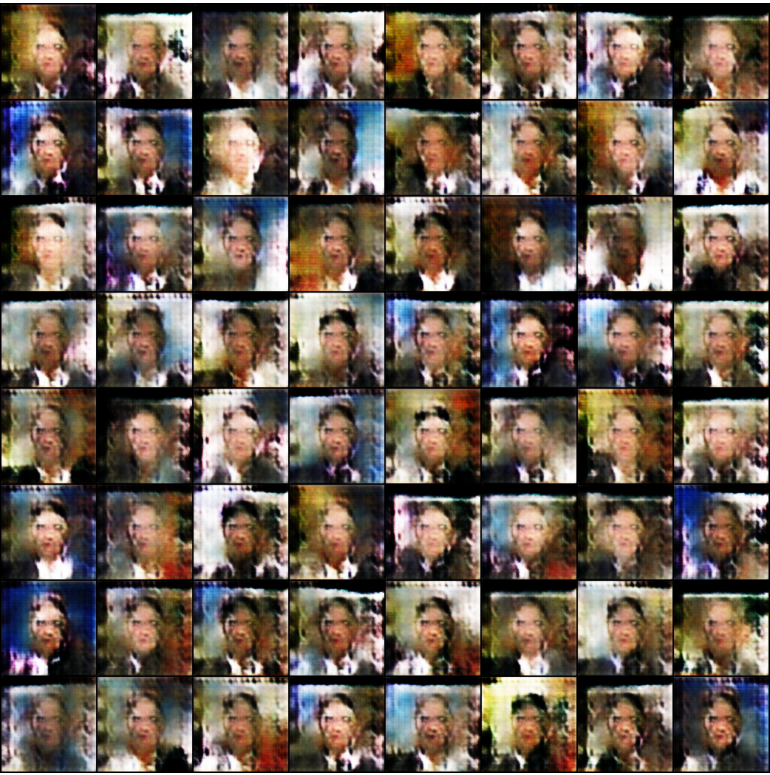
\includegraphics[width=0.8\textwidth]{./images/GAN.png}
\caption{GAN生成的图像}
\label{fig:GAN}
\end{figure}
\subsubsection{激活函数选择}
首先。我就进行了最直观的尝试,将判别器的激活函数由sigmoid改为tanh,并观察生成的图像的情况,其他模型参数没有具体变动。根据原理层面的推测和过往文章中给出的推测,应该可以比较明显地改善最后的生成效果,判别器则没必要做出类似的改变。\par
\begin{table}[htbp]
\centering
\caption{tanhGAN生成器网络结构}
\label{tab:gen_tanhgan}
\begin{tabular}{cccc}
\toprule[1.5pt]
\textbf{层类型} & \textbf{输入参数维度} & \textbf{输出参数维度} & \textbf{激活函数} \\
\midrule[1.5pt]
Linear输入层 & 128$\times$128$\times$3 & 256$\times$265$\times$3 & ReLU \\
Linear隐层1 & 256$\times$256$\times$3 & 128$\times$128$\times$3 & ReLU \\
Linear隐层2 & 128$\times$128$\times$3 & 64$\times$64$\times$3 & ReLU \\
Linear输出层 & 64$\times$64$\times$3 & 128$\times$128$\times$3 & tanh \\
\bottomrule[1.0pt]
\end{tabular}
\end{table}
最后呈现出的结果便是如图\ref{fig:GAN_tanh}所示的样子。通过仔细观察,我们可以明显看出生成的人脸图像相较于初始的随机噪声,已经有了显著的改善。人脸的轮廓变得更加清晰,展现出了较为明显的结构特征。这一变化表明,生成器对人脸的整体结构有了初步的理解,并能从噪声中提取出一些基础的面部特征。而且五官的位置也变得相对明确,虽然仍然存在一定的模糊性,但眼睛、鼻子、嘴巴等基本构成已经显现出来,说明生成器在学习的过程中,已经开始捕捉到人脸的关键信息。与此同时,背景的色块也展现出明显的差异,原本完全混沌的背景已经开始展现出一定的层次感,这暗示着生成器对复杂噪声的适应能力逐渐增强。总体来看,模型已经能够初步地区分并产生与噪声相对立的有意义的图像内容。因此可以认为,$tanh$这样的薄尾的归一化不仅稳定了生成图像中的细节,也有效地帮助了模型在图像细节的恢复中,保持了较高的稳定性,尤其是在人脸的轮廓和五官的生成方面,表现出了明显的优势。这些初步的进展为后续的训练和生成过程奠定了坚实的基础。后续也将初步保持选用$tanh$。
\begin{figure}[H]
\centering
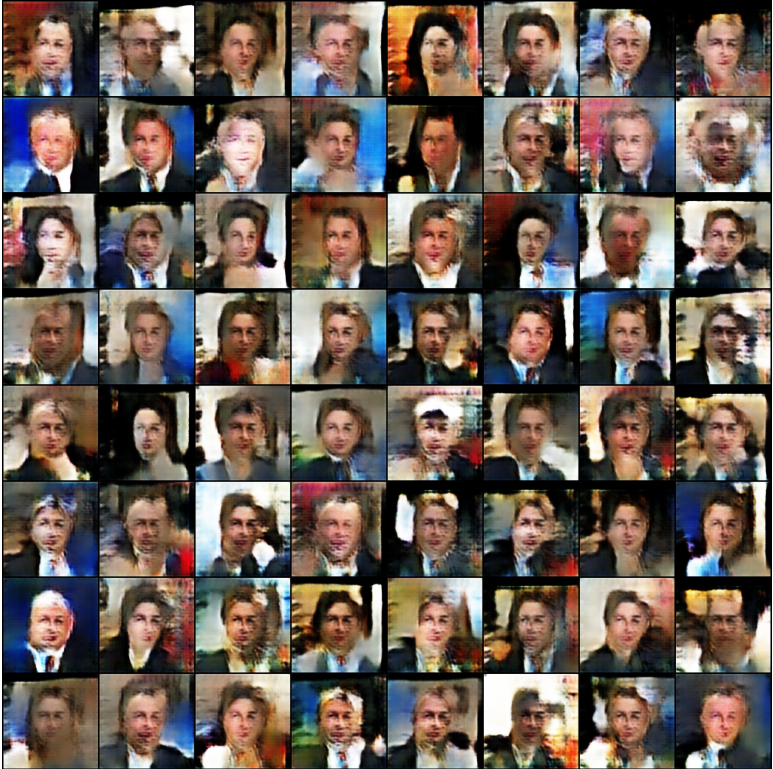
\includegraphics[width=0.8\textwidth]{./images/GAN_tanh.png}
\caption{GAN生成的图像}
\label{fig:GAN_tanh}
\end{figure}
\subsubsection{卷积层的引入}

\subsubsection{多阶段优化器的选择}

\section{模型的优势}


\section{模型的不足}



\bibliographystyle{plain}
\bibliography{references}

\end{document}

